\documentclass[12pt,a4paper]{article}
\usepackage{multirow}
\usepackage{bm}
\usepackage{AMSFONTS}
\usepackage{amssymb}
\usepackage{latexsym}
\usepackage{graphicx}
\usepackage{subfigure}
\usepackage{ hyperref}
\usepackage{biblatex}
\bibliography{bibliography}

\textwidth 6.5in
\textheight 9in
\topmargin 1pt
\linespread{1.5}
\oddsidemargin 0pt
\begin{document}
\title{\huge{HW1 }}


\author{Yilun Zhang}
\newtheorem{coro}{\hskip 2em Corollary}[section]
\newtheorem{remark}[coro]{\hskip 2em Remark}
\newtheorem{propo}[coro]{\hskip 2em  Proposition}
\newtheorem{lemma}[coro]{\hskip 2em Lemma}
\newtheorem{theor}[coro]{\hskip 2em Theorem}
\newenvironment{prf}{\noindent { proof:} }{\hfill $\Box$}
\date{\today}
\maketitle
\section*{Exercise 1}
Since $P$ is a projector, $P^2=P$, then \[
||P||_2=||P^2||_2\le||P||_2^2
\]
Therefore,$||P||_2\ge1$ 
Now, going to show that equality holds iff $P$ is an orthogonal projector.

If $P$ is an orthogonal projector, $P'=P$ and suppose $P$ has SVD $P=U\Sigma V'$
\[\sigma=||P||_2=||P^2||_2=||PP'||_2=||\Sigma^2||_2=\sigma^2
\]
where $\sigma$ is the largest eigen value of $P$. Therefore, $\sigma=1$

Suppose $P$ is not orthogonal. Then exist $a$, $a\not\in range(P)$ and $a\perp range(I-P)$\[
||Pa||_2=||a+(P-I)a||_2>||a||_2
\]
Then\[
||P||_2=\sup_{||a||_2=1}||Pa||_2>\sup_{||a||_2=1}||a||_2=1
\]
By contradiction $P$ is orthogonal.

\section*{Exercise 2}
Taking derivative wrt $x$, we got the normal equation\[
A'Ax=A'b\Rightarrow A'r=0
\]
Therefore the problem of minimization is equavalent to 
$$\begin{array}{ccc}
A'r&=& 0\\
Ax+r&=& b
\end{array}$$

\[
\min_x\{\frac{1}{2}||Ax-b||^2+\frac{1}{2}\delta^2||x||^2+c'x\}=\min_x\{\frac{1}{2}(Ax-b)'(Ax-b)+\frac{1}{2}\delta^2x'x+c'x\}
\]

Taking derivative wrt $x$, and set it to 0:\[
A'Ax-A'b+\delta^2x+c=0
\]
Therefore the problem is equivalent to $$\begin{array}{ccc}
A'r+\delta^2x&=& -c\\
Ax+r&=& b
\end{array}$$
\[\left(
\begin{array}{cc}
I&A\\
A^T&\delta^2I
\end{array}\right)\left(
\begin{array}{c}
r\\
x
\end{array}\right)=\left(
\begin{array}{c}
b\\
-c
\end{array}\right)
\]
\section*{Exercise 3}
Suppose that $m>n$ and $A$ has full rank so that $A^TA$ is invertible. $A=U\Sigma V^T$ is the full SVD, ie, $U$ is $m\times m$ square matrix and $V$ is $n\times n$ square matrix. $U^TU=UU^T=I_m$, $V^TV=VV^T=I_n$.And $\Sigma=\left(\begin{array}{c}
L\\0
\end{array}\right)$, where $L=diag(\lambda_1,\cdots,\lambda_n)$, $\lambda_i$ are singular values of A
\subsection*{1}
\begin{eqnarray*}
(A^TA)^{-1}&=&(V\Sigma^TU^TU\Sigma V^T)^{-1}\\
&=&(V\Sigma^T\Sigma V^T)^{-1}\\
&=&(VL^2 V^T)^{-1}\\
&=&VL^{-2}V^T
\end{eqnarray*}
$L^{-2}=diag(\lambda_1^{-2},\cdots,\lambda_n^{-2})$
\subsection*{2}
\begin{eqnarray*}
	(A^TA)^{-1}A^T&=&VL^{-2}V^T V\Sigma^TU^T\\
	&=&VL^{-2}\Sigma^TU^T\\
	&=&V\left(\begin{array}{cc}
		L^{-1}&0
	\end{array}\right)U^T
\end{eqnarray*}
\subsection*{3}
\begin{eqnarray*}
	A(A^TA)^{-1}&=&U\Sigma V^T VL^{-2}V^T \\
	&=&U\Sigma L^{-2}V^T\\
	&=&U\left(\begin{array}{c}
		L^{-1}\\0
	\end{array}\right)V^T
\end{eqnarray*}

\subsection*{4}
\begin{eqnarray*}
	A(A^TA)^{-1}A^T&=&U\left(\begin{array}{c}
		L^{-1}\\0
	\end{array}\right)V^T V\Sigma^T U^T \\
	&=&U\left(\begin{array}{c}
		L^{-1}\\0
	\end{array}\right)\left(\begin{array}{cc}
	L & 0
\end{array}\right)U^T\\
&=& U\left(\begin{array}{cc}
	I & 0\\
	0 & 0
\end{array}\right)U^T
\end{eqnarray*}
\section*{Exercise 4}
Since $rank(A)=m$ then $dim(range(A))=m$, this implies $dim(null(A))=n-m$. So the dimension if solution space is n-m.

Suppose $x_0$ is a solution of $Ax=b$, and $x\in null(A)$, clearly $x_0+x$ is a solution of $Ax=b$. Then our problem becomes minimize $||x_0+x||_2$. Let $B$ be the basis of null(A). Then $x\in range(B)$, exist $v$, s.t $Bv=x$. 
\begin{eqnarray*}
\min_x||x_0+x||_2&=&\min_v||x_0+Bv||_2\\
&=&\min_v||x_0+Bv||_2\\
&=&\min_v||Bv-(-x_0)||_2
\end{eqnarray*}
This is of same form of regular least square problem in overdetermind system. Then we can easily get the solution like overdetermind system.
\subsection*{normal equation}
\[B'Bv=-B'x_0
\]
\subsection*{QR}
Assume $B=QR$, then
\[Rv=-Q^Tx_0
\]
\subsection*{SVD}
Assume $B=U\Sigma V^T$ is the full singular value decomposition
\[
\Sigma V^Tv=-U^Tx_0
\]
\section*{Exercise 5}
Declaration of reference: I'm new to MATLAB. The code of log-barrier penalty and generating plots consult \url{http://cvxr.com/cvx/examples/cvxbook/Ch06_approx_fitting/html/penalty_comp_cvx.html#source}
\begin{figure}
	
	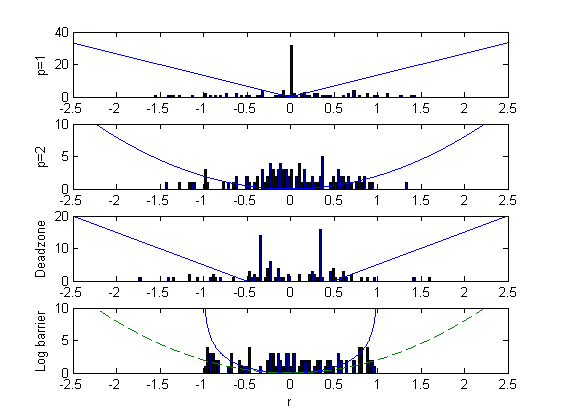
\includegraphics[width=\textwidth]{fig.png}
\end{figure}

\end{document} 